\section{Experiments}
\subsection{Problem description}
In order to validate the performance of the proposed algorithm, the warehouse facility location problem in Wuhan rail transit system is used as the benchmark instance in this paper.

There are eight rail transit lanes and each lane's material demands are known in advance.
The problem is to decide the optimal number of warehouse facility locations as well as the rail lanes they service respectively.
Table \ref{tab:tab1} contains the relative positions of the eight possible car depot locations that can be used to build warehouse facilities.
Eight warehouses need to be built before optimization, meaning each warehouse services one and only one rail lane.
For example, the position of 1(181, 231) indicates the first warehouse facility is located at $x$-axis of 181 and $y$-axis of 231.

\begin{table}[h!]
	\begin{center}
		\caption{Warehouse facilities relative positions}
		\label{tab:tab1}
		\begin{tabular}{cccc}
			\hline
			1 & 2 & 3 & 4 \\
			(181, 231) & (355, 105) & (442, 83) & (765, 275) \\
			\hline
			5 & 6 & 7 & 8 \\ 
			(422, 637) & (300, 563) & (287, 235) & (572, 605)\\
			\hline
		\end{tabular}
	\end{center}
\end{table}

Parameters of the proposed algorithm are set as follows: number of drones 100, number of larvae 200, size of queen bee ovary 100, number of iterations 200.
The warehouse facility location model described in this paper is implemented in C++ and 20 independent replications are run to obtain the optimal warehouse locations.
The computational results show that 4 warehouse facilities are enough to cover the demands from all rail lanes.
The warehouse coverage is illustrated in table \ref{tab:tab2}.
Figure \ref{fig:fig3} gives the graphical demonstration of the computational results.

\begin{figure}[h!]
	\begin{center}
		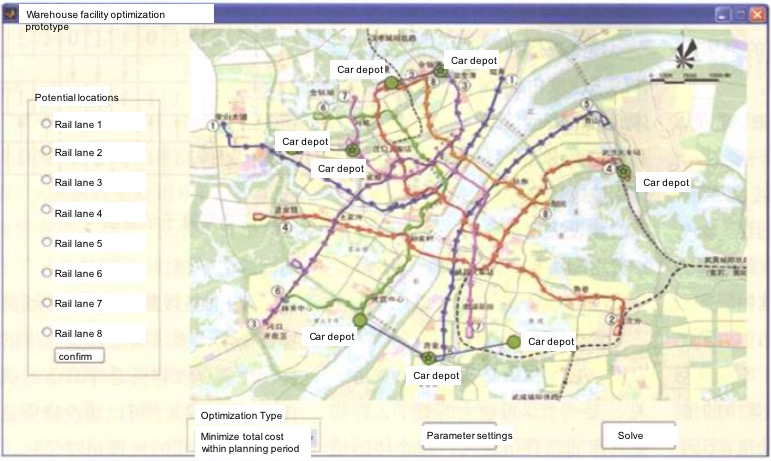
\includegraphics[width=0.8\linewidth]{sections/figure3.jpg}
		\caption{Warehouse facility locations after optimization}
		\label{fig:fig3}
	\end{center}
\end{figure}

\begin{table}[h!]
	\begin{center}
		\caption{Warehouse facility coverage settings}
		\label{tab:tab2}
		\begin{tabular}{cc}
			\hline
			Warehouse no. & rail lanes covered \\
			\hline
			1 & 2, 3\\
			2 & 4 \\
			3 & 5, 6, 8\\
			4 & 1, 7\\
			\hline
		\end{tabular}
	\end{center}
\end{table}

\subsection{Computational result comparison}
The average cost in 20 runs is 294,100,000, compared to original cost of 341,600,000.
A total of 47,500,000 is saved from the optimization exercise.
Figure \ref{fig:fig4} shows the cost comparison before and after optimization.

\begin{figure}[h!]
	\begin{center}
		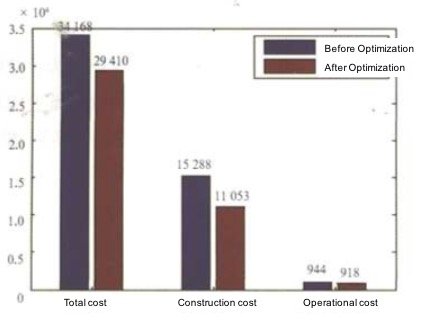
\includegraphics[width=0.8\linewidth]{sections/figure4.jpg}
		\caption{Cost comparison before and after optimization}
		\label{fig:fig4}
	\end{center}
\end{figure}

\subsection{Algorithm stability}
Figure \ref{fig:fig5} shows the algorithm stability for the 20 runs.
The $x$-axis represents the number of each individual run, and the $y$-axis indicates objective function value related to total cost.
The star in the graph indicates the best solution in the 20 runs, and the line represents the average value throughout the 20 runs.
It can be seen from the graph that the algorithm demonstrates great level of stability.

\begin{figure}[h!]
	\begin{center}
		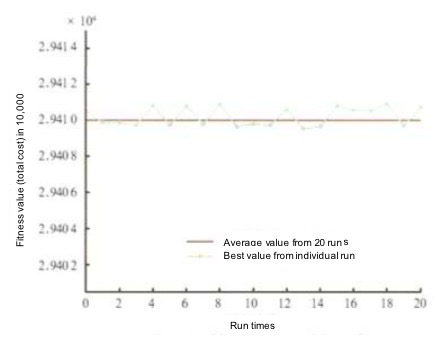
\includegraphics[width=0.8\linewidth]{sections/figure5.jpg}
		\caption{Illustration of algorithm stability in 20 runs}
		\label{fig:fig5}
	\end{center}
\end{figure}